%%%%%%%%%%%%%%%%%%%%%%%%%%%%%%%%%%%%%%%%%%%%%%%%%%%%%%%%%%%%%%%%%%%%%%%%%%%%%%%
%%%%%%%%%%%%%%%%%%%%%%%%%%%%%%%%%%%%%%%%%%%%%%%%%%%%%%%%%%%%%%%%%%%%%%%%%%%%%%%
%%%%  CHAPTER 6 
%%%%%%%%%%%%%%%%%%%%%%%%%%%%%%%%%%%%%%%%%%%%%%%%%%%%%%%%%%%%%%%%%%%%%%%%%%%%%%%
%%%%%%%%%%%%%%%%%%%%%%%%%%%%%%%%%%%%%%%%%%%%%%%%%%%%%%%%%%%%%%%%%%%%%%%%%%%%%%%
\chapter{Diagnostic tools I: Polarization phase-contrast imaging}

Experiments with ultracold atoms rely on a variety of very well established
measurement and diagnostic techniques~\cite{Making1999,Making2007}.  Most
measurement techniques are based on the possibility of imaging the column
density distribution of the sample \textit{in-situ} or after releasing it in
time-of-flight (TOF).  These include absorption imaging, fluorescence imaging,
and phase-contrast imaging.  More complicated techniques change the state of
the gas prior to imaging in order to gain access to other physical quantities.
These include, for example, Stern-Gerlach
separation in a magnetic field gradient, association of free atoms into
molecules using a Feshbach resonance, or band-mapping of atoms in an optical
lattice, just to name a few. 

From the raw images obtained after a measurement one has to implement analysis
and diagnostic tools, which extract the relevant physical quantities.  For
instance, the shape or size of the column density distribution
(\textit{in-situ} or after TOF) of a Fermi gas in a harmonic trap  can be used
to obtain its temperature. 
%, or the radial derivative of an \text{in-situ} column density distribution
%can be used to extract the compressibility of the gas ( we do this for a
%lattic gas in Chapter~\ref{chap:mott}). 

Over the course of this thesis we have elaborated and improved some of the
already established measurement and diagnostic techniques in the lab
(polarization phase-contrast imaging and Fermi gas thermometry).   We have also
developed new techniques not previously available in the lab (measurement of
double occupancies in an optical lattice using molecular association),  and
pioneered a new technique (spin sensitive Bragg scattering of light) to probe
the spin-ordering of atoms in lattices.  The following chapters are devoted to
the detailed explanation of those techniques that were improved or newly
developed for the work in this thesis.    

 
\section{Polarization phase-contrast imaging} 

Polarization phase-contrast imaging (PPCI) has been a workhorse at the Hulet
lab since the early days~\cite{Bradley1997,Dries2010}.  It was first analyzed
in the Ph.D. theses of Curtis Bradley~\cite{Bradley1996} and Cass
Sackett~\cite{Sackett1998}. It is used at various stages of our experiment to
measure the \textit{in-situ} column density of the dilute gas.   The general
goal of imaging is to obtain a quantitative measure of the density distribution
of the sample by analyzing the intensity, phase and polarization profiles of
light that has gone through it.    The widely used absorption imaging technique
looks at the intensity attenuation profile for a resonant, or nearly resonant
laser beam.   On the other hand, light with a larger detuning is used for PPCI.
Rather than looking for attenuation of the intensity, the information about the
density of the gas can be extracted from the phase profile of the transmitted
beam.   Techniques that rely on phase change are referred to as dispersive, in
contrast to absorptive techniques which measure intensity changes. 

Traditionally, a two-level model of the atom has been used in our lab in order
to relate the measured phase profile to an atomic density.  In an optical
lattice with site spacing $a=532\,$nm, a density of one atom per site
corresponds to 6.64$\times10^{12}$\,cm$^{-3}$.  At these densities the detuning
from the atomic transition must be increased in order to avoid non-linearities
in the phase to density conversion,  which can occur if the phase change of the
electric field after going through the atom cloud is $>\pi/5$.   Typically, a
detuning $<100$~MHz is used for PPCI in our lab for samples of moderate
densities and the two-level model is sufficient to obtain the atomic density.
However, for some of our samples in the optical lattice and the optical dipole
trap (see Chapter~\ref{chap:setup-overview} for a description of the experimental
setup) we have had to increase it to several hundred MHz.  When the detuning
becomes comparable to the energy spacing between the excited state and other
fine-structure levels in the excited manifold, the contributions to the phase
change from these other states becomes non-negligible and must be taken into
account when calculating the atomic density distribution from the measured
phase profile. 

Here we derive the formulas that are used to convert phase-contrast to atomic
density including the effects from other fine-structure levels in the excited
state.  The treatment is separated into five parts: \vspace{-1em}
\begin{enumerate} 
 \item  We calculate how the
light is affected by the polarized atomic cloud.  This is done classically,
using Maxwell's equations and assuming that we know the polarization of the
medium.  

 \item We calculate the polarization of the
atomic cloud, which results from the oscillating electric field of the imaging
light acting as a perturbation on the atoms. We derive the form of the electric
susceptibility tensor, which determines the polarization response of the gas to
the oscillating field.  

 \item We evaluate the elements of the susceptibility tensor for the atomic
structure relevant to us, namely a spin-mixture of $^{6}$Li atoms at high
magnetic field. 

\item  We then proceed to derive expressions that relate the phase
profile of the transmitted beam to the column density of the cloud.  

 \item We  examine the general experimental setup which allows one to convert
the phase profile into an intensity profile that can be recorded on a CCD
camera.  
\end{enumerate}
\vspace{0.5em}

To start out with some context, Fig.~\ref{fig:levels} shows the energy level
structure relevant for our experiment.   We typically use a spin mixture of
hyperfine states $|1\rangle$ and $|2\rangle$ in the $F=1/2$ manifold of the
$2S_{1/2}$ ground state.   The magnetic field where we carry out our
experiments is usually $>300~$G, where the energy dependence of states is
linear with field.   The red lines in Fig.~\ref{fig:levels} indicate state
$|1\rangle$ and the excited state involved in  the imaging process. For a large
red detuning, the spacing between the $m_{J}=-1/2$ and $m_{J}=-3/2$ excited
states can be comparable to the detuning.   If blue-detuned light is used the
contributions from states other than $m_{J}=-3/2$ will be even more
significant. 
\begin{figure}
\centering
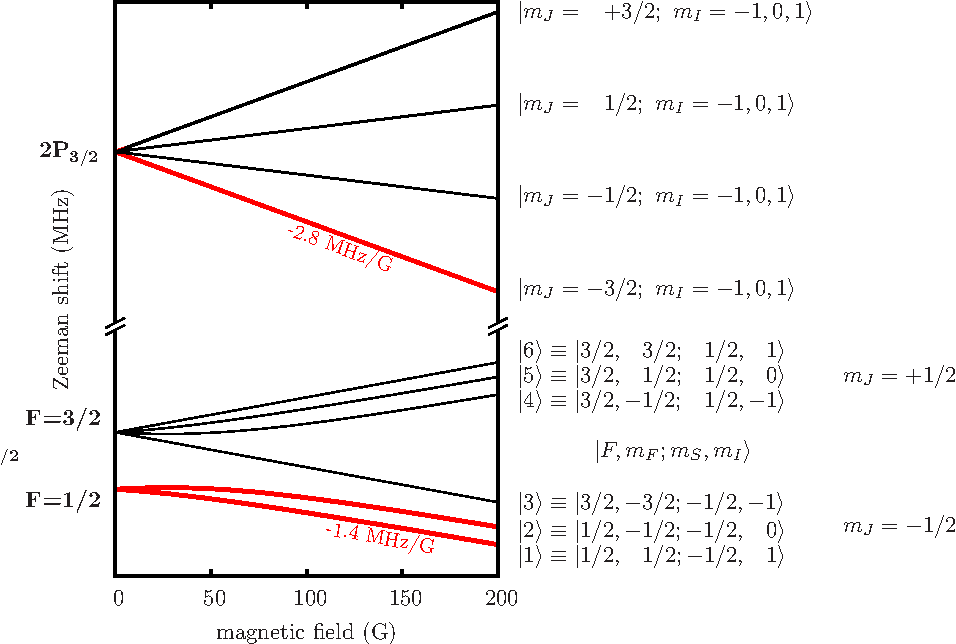
\includegraphics[width=0.85\textwidth]{../figures/phasecon/01eps.pdf}
\caption[Levels relevant for imaging.]{Level diagram relevant for imaging
transitions.  The levels relevant for imaging are highlighted in red. }
\label{fig:levels}
\end{figure}

 
\subsection{Transmission of light through a polarized gas} 

The electric field of the light that traverses the atomic cloud can be written
in general form (see Sec.~6.1 of~\cite{auzinsh2010optically}) as 
\begin{equation}
 \efield( \bv{r}, t ) = 
     \text{Re}\lbrace \efieldo e^{i(\bv{k}\cdot\bv{r} - \omega t + \varphi )} 
     [ \cos\phcChi \bv{\hat{e}}_{1} 
   +   \sin\phcChi e^{i\phi} \bv{\hat{e}}_{2} ] \rbrace 
  \label{eq:efield-param}
\end{equation}
where $\bv{\hat{e}}_{1,2}$ are two orthogonal unit vectors perpendicular to the
wave vector $\bv{k}$ and perpendicular to each other, $\phi$ is the relative
phase between the two polarization components,  $\efieldo$ is the electric
field amplitude, $\varphi$ is an overall phase,  and $\phcChi$ is related to
the angle of the polarization ellipse with respect to $\bv{\hat{e}}_{1}$ and
$\bv{\hat{e}}_{2}$. 

The wave equation in a dielectric medium can be obtained from Maxwell's
equations\footnote{Note that Gaussian units are used in this section, following
the treatment in~\cite{auzinsh2010optically}}, and is given by 
\begin{equation}
 \nabla^{2} \efield 
 -\frac{1}{c^{2}} \frac{\partial^{2} \efield } {\partial t^{2}} 
  = \frac{4\pi}{c^{2}} \frac{\partial^{2} \dpol }{\partial t^{2} } .
\end{equation} 
Here, the medium polarization $\dpol$ (which is induced by the imaging light)
corresponds to the dipole moment per unit volume.   If we know the dipole
moment of a single atom $\langle d \rangle$ then \begin{equation}
 \dpol = n \langle d \rangle 
\end{equation}
where $n$ is the density of the gas.

Just as the electric field was parameterized in Eq.~\ref{eq:efield-param}, the
polarization can be written in terms of the four real parameters
$P_{i}$ as 
\begin{equation}
 \dpol = \text{Re} \lbrace e^{i(\bv{k}\cdot\bv{r} - \omega t + \varphi) }
   [(P_{1} - i P_{2}) \bv{\hat{e}}_{1} + ( P_{3} - i P_{4}) \bv{\hat{e}}_{2} ] \rbrace
  \label{eq:pol-param}
\end{equation}

Using the oscillatory time dependence of \efield\ and \dpol\ the wave equation
is reduced to 
\begin{equation}
   \frac{ \partial^{2} \efield}{\partial \ell^{2} }  + k^{2} \efield = - 4 \pi k^{2} \dpol
\end{equation}
where $\ell$ is the distance along the light propagation direction. 

The parameterized electric field and polarization are plugged into the wave
equation,  and one proceeds to neglect terms that are of second order in the
derivatives of the electric field parameters.  This is justifiable, as long as the
fractional change of the parameters is small over distances of the order of the
imaging light wavelength, which is certainly the case for our dilute atom
cloud.  The resulting expressions for the change of the field parameters per
unit distance are:
\begin{equation}
\begin{split}
 \frac{1}{\efieldo} \frac{d \efieldo }{ d \ell} & = \   
     \frac{2\pi \omega}{\efieldo c} ( P_{2} \cos\phcChi + P_{4} \sin\phcChi ) \\ 
 \frac{ d \varphi }{d \ell} & = \ 
     \frac{2\pi\omega}{\efieldo c} \left( \frac{ P_{1} }{\cos\phcChi} \right) \\
 \frac{ d \phcChi}{ d \ell} & = \
     \frac{2\pi\omega}{\efieldo c} ( -P_{2} \sin\phcChi + P_{4} \cos\phcChi ) \\
 \frac{ d \phi}{ d \ell} & = \ 
     \frac{2\pi\omega}{\efieldo c }
     \left(  \frac{ P_{1}\sin\phcChi - P_{3}\cos\phcChi }{ \sin\phcChi\cos\phcChi } \right)
 \label{eq:diff-param}
\end{split}
\end{equation} 
 
     
    
\subsection{Polarization of the cloud}  


If we can calculate the electric
dipole moment induced on one atom, $\langle \bv{d}\, \rangle$, and if we know
the density of the cloud, $n(\vec{r})$, then we can simply write the induced
polarization as 
\begin{equation}
 \dpol(\bv{r}) = \langle \bv{d}\, \rangle n(\bv{r}) 
\end{equation}

An ensemble of atoms (in which each atom may be in a different quantum state) is
best described using the density matrix, which is defined as \begin{equation}
  \rho = \frac{1}{N} \sum_{i=1}^{N} | \psi_{i} \rangle \langle \psi_{i} | 
\end{equation}
where the $i^{\text{th}}$ atom in the ensemble is in state $|\psi_{i}\rangle$.
The expectation value of the electric dipole moment is then given by 
\begin{equation}
\begin{split}
   \langle \bv{d}\, \rangle  & = \text{Tr} ( \rho \bv{d} )  \\
   & = \sum_{mn} \rho_{mn} \langle n | \bv{d} | m \rangle
\end{split} 
\end{equation} 
Since the dipole operator only couples states of different parity, the terms
that contribute to this sum correspond to the pair $m,n$ being a ground and
excited state pair.   

The equation of motion for the density matrix (Liouville equation) follows from
the Schrodinger equation for the $|\psi_{i}\rangle$, and including the
spontaneous decay of the excited state~\cite{auzinsh2010optically} can be
written as
\begin{equation}
  i \hbar \dot{\rho} = 
  [H, \rho] - \frac{i\hbar}{2}\lbrace \hat{\Gamma}, \rho \rbrace + i\hbar\text{Tr}( F \rho ) 
\end{equation}
where $\hat{\Gamma}$ is the relaxation matrix, a diagonal matrix with the decay
rate of each state on the diagonal (see Sec.~5.5
in~\cite{auzinsh2010optically}), and $F$ is the spontaneous emission operator
(see Sec.~12.1 in~\cite{auzinsh2010optically}).  The Hamiltonian
$H$ can be split into a diagonal part, $H_{0}$, which includes the
level structure of the atom in the presence of a magnetic field, and the time
dependent perturbation from the electric field $\hbar V$:
\begin{equation}
  H = H_{0} + \hbar V
\end{equation}

The matrix element $\rho_{ge}$, where $g$, $e$ represent a ground and an
excited state respectively, can be plugged into the Liouville equation to
obtain
\begin{equation}
\begin{split}
  \dot{\rho}_{ge}  & =  
   \frac{1}{i\hbar} \langle g | [ H_{0}, \rho ] | e \rangle  
 - i \langle g | [ \hbar V, \rho ] | e \rangle 
 - \frac{1}{2}\langle g | \lbrace \hat{\Gamma}, \rho \rbrace | e \rangle 
 + \langle g | \text{Tr}( F \rho ) | e \rangle  \\
 & = -i \tilde{\omega}_{ge}  \rho_{ge}  
     -i \sum_{p}\left( V_{gp} \rho_{pe} - \rho_{gp}V_{pe} \right) 
     +  \sum_{rs} F_{ge}^{sr} \rho_{rs}
\end{split} 
\end{equation}
where 
\begin{equation}
  \tilde{\omega}_{ge} = (E_{g} - E_{e})/\hbar - i \Gamma_{e} /2 
\end{equation}
We notice that $F_{ge}^{sr} = 0$, since $F$ is only nonzero if the lower
indices are both ground states and the upper indices are both excited states.
So we are left with 
\begin{equation}
  \dot{\rho}_{ge}  =  
     -i \tilde{\omega}_{ge}  \rho_{ge}  
     -i \sum_{p}\left( V_{gp} \rho_{pe} - \rho_{gp}V_{pe} \right) 
\end{equation}

At this point we switch to the rotating frame (see Sec.~10.2.2
in~\cite{auzinsh2010optically}), in which the density matrix $\tilde{\rho}$ can
be obtained from
\begin{equation}
 \tilde{\rho} = U^{\dagger} \rho U
\end{equation} 
where $U$ is a unitary diagonal matrix with entries given by 
\begin{equation} 
  U_{mm} = \begin{cases} 
   1 & \text{if  $m$ is a ground state} \\
   e^{i(\bv{k}\cdot\bv{r}-\omega t)} & \text{if $m$ is an excited state} 
  \end{cases}
\end{equation}
We thus have $\tilde{\rho}_{ge} = \rho_{ge} e^{i(\bv{k}\cdot\bv{r}-\omega t)}$,
and the equation of motion for the $\rho_{ge}$ matrix element in the rotating
frame is
\begin{equation}
\begin{split}
  \dot{\tilde{\rho}}_{ge} & = 
     -i\omega \tilde{\rho}_{ge} + \dot{\rho}_{ge} e^{i(\bv{k}\cdot\bv{r}-\omega t)} \\
     &  =  
     -i\omega \tilde{\rho}_{ge} + 
      \left[ 
     -i \tilde{\omega}_{ge}  \rho_{ge}  
     -i \sum_{p}\left( V_{gp} \rho_{pe} - \rho_{gp}V_{pe} \right) 
      \right] e^{i(\bv{k}\cdot\bv{r}-\omega t)}  \\ 
     &  =  
     -i \tilde{\rho}_{ge}\tilde{\omega}'_{ge}   
     -i \sum_{p}\left( V_{gp} \rho_{pe} - \rho_{gp}V_{pe}\right)  e^{i(\bv{k}\cdot\bv{r}-\omega t)}   
\end{split} 
\end{equation}
where 
\begin{equation}
  \tilde{\omega}'_{ge} = \omega + (E_{g} - E_{e})/\hbar - i \Gamma_{e}/2 
   \equiv  \Delta_{ge} - i \Gamma_{e}/2 
\end{equation}
We recall that the interaction term is of the electric dipole type: 
\begin{equation} 
  \hbar V = -\bv{d} \cdot \efield 
    =  -\bv{d} \cdot \efieldo 
          \text{Re}[ \epspol e^{i(\bv{k}\cdot\bv{r} - \omega t )} ]
    =  -\bv{d} \cdot 
           \frac{  \efieldo ( \epspol e^{i(\bv{k}\cdot\bv{r} - \omega t)} 
                + \epspol^{*} e^{-i(\bv{k}\cdot\bv{r}-i\omega t)} )}{2} .
\end{equation}
Introducing this in the equation of motion for $\tilde{\rho}_{ge}$, 
neglecting the rapidly oscillating terms, and making use of the fact that the
wavelength of the light is much larger than the extent of the atom (so that the
spatially dependent exponential can be taken outside of matrix elements) one
gets to 
\begin{equation} 
\begin{split}
  \dot{\tilde{\rho}}_{ge} & =  
     -i \tilde{\rho}_{ge}\tilde{\omega}'_{ge}   
     + \frac{i}{2\hbar} \sum_{p}\left[ \bv{d}_{gp} \rho_{pe} 
     - \rho_{gp}\bv{d}_{pe}\right] \cdot \efieldo \epspol^{*}
\end{split} 
\end{equation}
which has a steady-state solution given by 
\begin{equation} 
  \tilde{\rho}_{ge}  = \frac{1}{2 \hbar\tilde{\omega}'_{ge} }  
       \sum_{p}\left[ \bv{d}_{gp} \rho_{pe} 
     - \rho_{gp}\bv{d}_{pe}\right] \cdot \efieldo \epspol^{*}
\end{equation}
Finally, we neglect coherences and populations in the excited states
($\rho_{ee'}=0$) and coherences in the ground states ($\rho_{gg'}=0$ if $g\neq
g'$).   This can be justified since the perturbation is weak and is not
expected to modify the initial excited state populations (which are zero).
Furthermore, coherences between ground states $g\neq g'$ can only be expected
if there is  population in the excited state: these coherences
can only develop is there is excitation from one ground state and then
spontaneous or stimulated emission to a different ground state, so they
can be neglected in the weak perturbation limit.  The final result is 
\begin{equation} 
  \tilde{\rho}_{ge} 
  =  -\frac{\bv{d}_{ge} \cdot \efieldo \epspol^{*}  }
       {\hbar (2 \Delta_{ge} - i \Gamma )} \rho_{gg} 
\end{equation}
%\begin{equation} 
%  \Rightarrow  \ \ \ 
%  \rho_{ge}  = -\frac{1}{2 \tilde{\omega}'_{ge} }  
%       (\bv{d}_{ge} \cdot \efield) e^{i\omega t}
%\end{equation}
which after plugging back into the equation for the expectation value of the dipole
moment gives 
\begin{equation}
\begin{split}
   \langle \bv{d}\, \rangle 
   & = \sum_{ge} 2 \text{Re}[ \rho_{ge} \bv{d}_{eg} ] \\
   & = \sum_{ge} 2 \text{Re}[ \tilde{\rho}_{ge}e^{-i(\bv{k}\cdot\bv{r}-\omega t)}\bv{d}_{eg} ]   \\
   & = \sum_{ge} \rho_{gg}\text{Re}[ 
 -\frac{\bv{d}_{ge} \cdot \efieldo \epspol^{*} }{ \hbar( \Delta_{ge} + i \Gamma/2 )} 
   e^{-i(\bv{k}\cdot\bv{r} - \omega t) } 
 \bv{d}_{eg} ]   \\
   & \equiv \sum_{ge}  \rho_{gg} \text{Re}[ 
 -\frac{\bv{d}_{eg} \cdot \efieldo \epspol }{ \hbar( \Delta_{ge} -i \Gamma/2 ) } 
   e^{i(\bv{k}\cdot\bv{r} - \omega t) } 
 \bv{d}_{ge} ]   \\
   & = \sum_{ge}  \rho_{gg}  \text{Re}[ 
 -\frac{\bv{d}_{eg} \cdot \tilde{\efield} }{ \hbar(  \Delta_{ge} -i \Gamma/2 ) } 
 \bv{d}_{ge} ]   \\
\end{split} 
\end{equation}
where in the last line $\tilde{\efield}= \efieldo \hat{\bv{\varepsilon}}
e^{i(\bv{k}\cdot\bv{r} - \omega t)}$ is the complex electric field vector (not
to be confused with the actual electric field vector which is a real quantity).

Labeling the cartesian components of $\bv{d}$ with Greek upper indices and
implying sums over repeated Greek indices (Einstein notation), we have  
\begin{equation}
\begin{split}
   \langle d^{\mu} \rangle
   & = \sum_{ge}   \rho_{gg}  \text{Re}[ -\frac{d_{eg}^{\nu} \tilde{\mathcal{E}}^{\nu}  d_{ge}^{\mu} }
      { \hbar(\Delta_{ge} - i\Gamma/2) }    ] \\
   & = \text{Re}\left[ \left( \sum_{ge}- \rho_{gg} \frac{d_{eg}^{\nu}   d_{ge}^{\mu}  }
       { \hbar(\Delta_{ge} - i\Gamma/2) }   
       \right)  \tilde{\mathcal{E}}^{\nu} \right] 
\end{split}
\end{equation}
and from here we can write 
\begin{equation}
   \dpol = \text{Re}\left[ \ts{\chi} \tilde{ \efield }  \right] \\
\end{equation}
where we have defined the electric susceptibility tensor as
\begin{equation}
\begin{split}
   \chi_{\mu\nu}
   & = - \frac{n}{\hbar} \sum_{ge}\rho_{gg} \frac{d_{eg}^{\nu}   d_{ge}^{\mu}  }
       { \Delta_{ge} - i\Gamma/2 } \\ 
   & = - \frac{n}{\hbar} \sum_{ge}\rho_{gg} 
   \frac{\langle e | d^{\nu} | g \rangle \langle g | d^{\mu} | e \rangle } 
       { \Delta_{ge} - i\Gamma/2 } 
\end{split} 
\end{equation}


\subsection{Susceptibility for $^{6}$Li atoms at high magnetic field}

Going back to the parameterization scheme for the electric field and the medium
polarization, introduced in Eqs.~\ref{eq:efield-param},\ref{eq:pol-param}, we
can identify\footnote{ The reader is reminded that $\ts{\chi}$ is a tensor and,
for instance, the product $\ts{\chi} \bv{\hat{e}}_{1}$ may have components
along both $\bv{\hat{e}}_{1}$ and $\bv{\hat{e}}_{2}$.}:
\begin{equation}
   (P_{1} - i P_{2}) \bv{\hat{e}}_{1} + ( P_{3} - i P_{4}) \bv{\hat{e}}_{2} 
 =   \efieldo \ts{\chi} 
     [  \cos\phcChi  \bv{\hat{e}}_{1} 
   + \sin\phcChi e^{i\phi}  \bv{\hat{e}}_{2} ] 
\end{equation}

Using  
$\bv{\hat{e}}_{1} = \left[ \begin{smallmatrix}  1 \\ 0 \end{smallmatrix} \right]$
and 
$\bv{\hat{e}}_{2} = \left[ \begin{smallmatrix}  0 \\ 1 \end{smallmatrix} \right]$
this can be written in matrix form as 
\begin{equation}
 \left[ \begin{matrix}  P_{1}-iP_{2} \\ P_{3}-iP_{4} \end{matrix} \right]
  =  \efieldo 
 \left[ \begin{matrix}
     \chi_{11} & \chi_{12} \\ \chi_{21} & \chi_{22} 
 \end{matrix} \right]
 \left[ \begin{matrix}
      \cos\phcChi \\
      \sin\phcChi e^{i\phi}
 \end{matrix} \right]
\label{eq:polmatrix}
\end{equation}

At this point we have to make a choice for the real space orientation of the
vectors $\bv{\hat{e}}_{1,2}$.  In our imaging setup the magnetic field is
oriented along the $z$ axis, and the probe beam propagates along $y$,
perpendicular to the magnetic field.   The polarization of the light lies on
the xz plane, so we will assign $\bv{\hat{e}}_{1} = \bv{\hat{x}}$ and
$\bv{\hat{e}}_{2} = \bv{\hat{z}}$, and we will evaluate the corresponding
components of the electric susceptibility tensor: $\chi_{xx}$, $\chi_{xz}$,
$\chi_{zx}$, and $\chi_{zz}$.

The first thing to notice is that the off-diagonal components of the
susceptibility vanish.  This is because the $x$ and $z$ components of the
dipole cannot couple to the same excited state (due to the dipole transition
angular momentum projection selection rules).   For the diagonal components we
will need to evaluate the matrix elements $ | \langle e | d_{i} | g \rangle
|^{2} $ for $i=x,z$,  which can be expressed in terms of the spherical basis
components of the dipole moment, $d_{q}$, as 
\begin{align}
|\langle e | d_{i} | g \rangle|^{2} & =  \sum_{q} |\bv{\hat{e}}_{i}\cdot \bv{\hat{e}}_{q}|^{2} 
 | \langle e | d_{q} | g \rangle | ^{2} 
\end{align}

The relevant quantum numbers for the ground and excited states are
\footnote{We omit the $J$ subscript in $m_{J}\equiv m$ for simplicity.}
\begin{align}
|g\rangle & = | R_{g}\, L_{g}\,S_{g}\,J_{g}\,m_{g} \rangle \\
|e\rangle & = | R_{e}\, L_{e}\,S_{e}\,J_{e}\,m_{e} \rangle 
\end{align}
where the labels $R,L,S,J,m$ refer to the radial quantum number, orbital
angular momentum, spin, total angular momentum, and projection on $z$-axis of
total angular momentum, respectively.  At the field of interest, the nuclear
spin and its projection are decoupled from the angular momentum of the
electron,  so they do not play any role in imaging, which is an electric dipole
process.  In our experiment, we typically have atoms in an incoherent spin
mixture of states $|1\rangle$ and $|2\rangle$. Looking back at the energy level
diagram in Fig.~\ref{fig:levels}, both of those states have $m_{J}=-1/2$, so
one can drive transitions from either of them to excited states with
$m_{J}=-3/2, -1/2, +1/2$.  In what follows we refer to those excited states
$|e\rangle$ as $|-\rangle$, $|\pi\rangle$, and $|+\rangle$ respectively. 

 
To evaluate $ | \langle e | d_{q} | g \rangle | ^{2} $, we use the
Wigner-Eckart theorem(see Sec.~5.4.1 of ~\cite{edmonds1996angular}) to make the
$J$, $m_{J}$ selection rules explicit in a 3$j$-symbol.  This results in  
\begin{align}
|\langle e | d_{q} | g \rangle|^{2} & = \begin{pmatrix} J_{e} & 1 & J_{g} \\ -m_{e} & q & m_{g} \end{pmatrix}^{2}
|\langle R_{e}\, L_{e}\,S_{e}\,J_{e} || d || R_{g}\, L_{g}\,S_{g}\,J_{g} \rangle|^{2}
\end{align}
which defines the reduced matrix element $\langle R_{e}\, L_{e}\,S_{e}\,J_{e} || d || R_{g}\, L_{g}\,S_{g}\,J_{g} \rangle$. 

The rate of spontaneous decay from the excited to the ground state is given by~\cite{budker2004atomic} 
\begin{equation}
\begin{split}
 \Gamma  = & \frac{4\omega_{0}^{3} }{3\hbar c^{3}} \sum_{J_{g}, m_{g} } 
 \begin{pmatrix} J_{e} & 1 & J_{g} \\ -m_{e} & q & m_{g} \end{pmatrix}^{2}
  |\langle R_{e}\, L_{e}\,S_{e}\,J_{e} || d || 
           R_{g}\, L_{g}\,S_{g}\,J_{g} \rangle|^{2}   \\
         = &  \frac{4\omega_{0}^{3} }{3\hbar c^{3}}  \frac{|\langle R_{e}\, L_{e}\,S_{e}\,J_{e} || d || 
           R_{g}\, L_{g}\,S_{g}\,J_{g} \rangle|^{2} }
       { 2J_{e} + 1 }
\end{split}
\end{equation}
and since $J_{e}=3/2$
\begin{equation}
\Rightarrow \ \ \ \ 
|\langle R_{e}\, L_{e}\,S_{e}\,J_{e} || d || R_{g}\, L_{g}\,S_{g}\,J_{g} \rangle|^{2} 
    =  \Gamma \frac{ 3\hbar c^{3}}{ \omega_{0}^{3} }  
    =  \Gamma \frac{ 3\hbar \lambda^{3}}{ 8 \pi^{3}}
\end{equation}
We thus have
\begin{align}
|\langle e | d_{q} | g \rangle|^{2} & = \begin{pmatrix} J_{e} & 1 & J_{g} \\ -m_{e} & q & m_{g} \end{pmatrix}^{2}
    \frac{ 3\hbar \Gamma \lambda^{3}}{ 8 \pi^{3}}
\end{align}
and for the cartesian component of the dipole moment
\begin{align}
|\langle e | d_{i} | g \rangle|^{2} & =  \sum_{q} |\bv{\hat{e}}_{i}\cdot \bv{\hat{e}}_{q}|^{2} \begin{pmatrix} J_{e} & 1 & J_{g} \\ -m_{Je} & q & m_{Jg} \end{pmatrix}^{2}
    \frac{ 3\hbar \Gamma \lambda^{3}}{ 8 \pi^{3}}
\end{align}

Going back to the $x$ and $z$ components of the dipole moment we have 
\begin{equation}
\begin{split}
   \chi_{xx}
   & = - \frac{n}{\hbar} \sum_{ge}\rho_{gg} 
   \frac{ |\langle g | d_{x} | e \rangle|^{2} } 
       { \Delta_{ge} - i\Gamma/2 } \\
   & = - \frac{n}{\hbar} \sum_{g} \rho_{gg} 
    \frac{ 3\hbar \Gamma \lambda^{3}}{ 8 \pi^{3}}
       \left( \frac{1}{\Delta_{-} - i \Gamma/2 } 
              |\bv{\hat{e}}_{x}\cdot \bv{\hat{e}}_{-}|^{2} 
              \begin{pmatrix} 3/2 & 1 & 1/2 \\ 3/2 & -1 & -1/2 \end{pmatrix}^{2} \right.  \\
   & \ \ \ \ \ \ \hspace{1.3in}\   +  
       \left. \frac{1}{\Delta_{+} - i \Gamma/2 } 
              |\bv{\hat{e}}_{x}\cdot \bv{\hat{e}}_{+}|^{2} 
              \begin{pmatrix} 3/2 & 1 & 1/2 \\ -1/2 & +1 & -1/2 \end{pmatrix}^{2} 
       \right) \\ 
   & = - \frac{n}{\hbar} \sum_{g} \rho_{gg} 
    \frac{ 3\hbar \Gamma \lambda^{3}}{ 8 \pi^{3}}
       \left( \frac{1/8}{\Delta_{-} - i \Gamma/2 } 
       +  
              \frac{1/24}{\Delta_{+} - i \Gamma/2 }  
       \right)  
\end{split} 
\end{equation}
\begin{equation}
\begin{split}
   \chi_{zz}
   & = - \frac{n}{\hbar} \sum_{ge}\rho_{gg} 
   \frac{ |\langle g | d_{z} | e \rangle|^{2} } 
       { \Delta_{ge} - i\Gamma/2 } \\
   & = - \frac{n}{\hbar} \sum_{g} \rho_{gg} 
    \frac{ 3\hbar \Gamma \lambda^{3}}{ 8 \pi^{3}}
              \frac{1}{\Delta_{\pi} - i \Gamma/2 } 
              |\bv{\hat{e}}_{z}\cdot \bv{\hat{e}}_{0}|^{2} 
              \begin{pmatrix} 3/2 & 1 & 1/2 \\ 1/2 & 0 & -1/2 \end{pmatrix}^{2} \\
   & = - \frac{n}{\hbar} \sum_{g} \rho_{gg} 
    \frac{ 3\hbar \Gamma \lambda^{3}}{ 8 \pi^{3}}
              \frac{1/6}{\Delta_{\pi} - i \Gamma/2 } 
\end{split} 
\end{equation}

In our experiment we have a balanced spin mixture of atoms in the ground states
$|1\rangle$ and $|2\rangle$,  so the sum over $\rho_{gg}$ can be carried out to
give 
\begin{equation}
\begin{split}
   \chi_{xx} & = - n  
    \frac{ 3 \Gamma \lambda^{3}}{ 8 \pi^{3}}
       \left( \frac{1/8}{\Delta_{-} - i \Gamma/2 } 
       +  
              \frac{1/24}{\Delta_{+} - i \Gamma/2 }  
       \right)  \\
   \chi_{zz} & = - n
    \frac{ 3 \Gamma \lambda^{3}}{ 8 \pi^{3}}
              \frac{1/6}{\Delta_{\pi} - i \Gamma/2 } 
\end{split}
\end{equation}
If we express the detunings in units of the linewidth we have 
\begin{equation}
\begin{split}
   \frac{2\pi\omega}{c} \chi_{xx} & = - n  
    \frac{ 3  \lambda^{2}}{ 2 \pi}
       \left( \frac{1/4}{2\Delta_{-} - i  } 
            + \frac{1/12}{2\Delta_{+} - i  }  
       \right) 
    \equiv - n \xi_{xx}
 \\
   \frac{2\pi\omega}{c} \chi_{zz} & = - n
    \frac{ 3  \lambda^{2}}{ 2 \pi}
              \frac{1/3}{2\Delta_{\pi} - i  } 
    \equiv - n \xi_{zz}
\label{eq:def-xis}
\end{split}
\end{equation}
Here we also have defined $\xi_{xx}$ and $\xi_{zz}$ which will be useful to 
simplify the notation later on.
 
%For the implementation of phase contrast imaging one detunes closest to the
%$|-\rangle$ state and being careful to keep $\Delta_{-} \gg \Gamma$. The
%$|-\rangle$ state is targeted since it is the one with the largest $3j$
%coefficient, thus the one that couples most strongly to the light.  At high
%magnetic field the $|+\rangle$ and $|\pi\rangle$ states are sufficiently far
%away that we always have  
%\begin{equation}
%  \frac{1}{\Delta_{-}} \gg \frac{1}{\Delta_{+}} , \frac{1}{\Delta_{\pi}}
%\end{equation}
%For now we will keep this in mind, because this will motivate some of the
%approximations we will make, but we will not drop the $+$ and $\pi$ terms
%altogether.  It will be seen that it is critical to keep these terms for
%accurate atom number counting when imaging at various detunings.   

From the matrix equation for the polarization parameters, 
Eq.~\ref{eq:polmatrix}, we see the correspondence 
\begin{equation}
\begin{split}
  P_{1} - i P_{2} & =  \efieldo \chi_{xx} \cos\phcChi \\
  P_{3} - i P_{4} & =  \efieldo \chi_{zz} \sin\phcChi e^{i\phi} 
        =   \efieldo \sin\phcChi \left[
            (\text{Re}\chi_{zz} \cos\phi - \text{Im}\chi_{zz}\sin\phi ) \right.\\
  & ~~~~~~~~~~~~~~~~~~~~~~~~~~~~~~~~~~~~~~ \left.
          +i(\text{Re}\chi_{zz} \sin\phi + \text{Im}\chi_{zz}\cos\phi ) \right]
\end{split}
\end{equation}
which results in
\begin{equation}
\begin{split}
  P_{1} &=  \efieldo \text{Re}\chi_{xx} \cos\phcChi \\
  P_{2} &= - \efieldo \text{Im}\chi_{xx} \cos\phcChi \\ 
  P_{3} &=  \efieldo \sin\phcChi 
            (\text{Re}\chi_{zz} \cos\phi - \text{Im}\chi_{zz}\sin\phi ) \\ 
  P_{4} &= - \efieldo \sin\phcChi
          (\text{Re}\chi_{zz} \sin\phi + \text{Im}\chi_{zz}\cos\phi ) \\ 
\end{split}
\end{equation}

\vspace{1em}
\subsection{ Change in field parameters due to atomic column density}

In terms of $\xi{xx}$ and $\xi{zz}$, the differential equations for the
electric field parameters, which were obtained in Eq.~\ref{eq:diff-param},
become 
\begin{equation}
\begin{split}
 \frac{1}{\efieldo} \frac{d \efieldo }{ d \ell} & = \   
     - [ \text{Im}\xi_{xx} \cos^{2}\!\phcChi 
       + (  \text{Re}\xi_{zz} \sin\phi + \text{Im}\xi_{zz}\cos\phi )  
             \sin^{2}\!\phcChi ] n(\ell)\\ 
 \frac{ d \varphi }{d \ell} & = \
      -\text{Re}\xi_{xx} n(\ell) \\ 
 \frac{ d \phcChi}{ d \ell} & = \ -\sin\phcChi\cos\phcChi
     ( \text{Im}\xi_{xx}
   - \text{Re}\xi_{zz} \sin\phi - \text{Im}\xi_{zz}\cos\phi ) n(\ell)\\
 \frac{ d \phi}{ d \ell} & = \
     -[ \text{Re}\xi_{xx} - \cos\phi \text{Re}\xi_{zz} 
       + \sin\phi \text{Im}\xi_{zz} ]n(\ell)
\end{split}
\end{equation}

If we knew the exact form of the density distribution of the gas $n(\ell)$ we
could solve these differential equations exactly,   but in fact, the goal of
this treatment is to do the converse. We want to find an expression for the
column density of the gas
\begin{equation}
  n_{\text{col}}  =  \int n(\ell) \text{d} \ell
\end{equation}

In general, the field parameters change from an initial value before the atoms
to a final value after the atoms.  To solve the differential equations for the
field parameters in terms of the column density, we will make the following
approximation 
\begin{equation}
  \int f(\phcChi, \phi) n(\ell) \,\text{d} \ell \approx 
       f(\phcChi_{i}, \phi_{i})  
       \int n(\ell) \text{d} \ell,
  \label{eq:phc-approx} 
\end{equation}
where the subscript $i$ denotes the value of the respective field parameter
before the light encounters the atom cloud.  This approximation assumes that
the field parameters $\zeta$ and $\phi$ will not change too much across the
extent of the cloud, and it leads to the following expressions for the change
in the field parameters:
\begin{equation}
\begin{split}
 \delta( \ln\efieldo ) & = \ 
     - [ \text{Im}\xi_{xx} \cos^{2}\!\phcChi_{i} 
       + (  \text{Re}\xi_{zz} \sin\phi_{i} + \text{Im}\xi_{zz}\cos\phi_{i} )  
             \sin^{2}\!\phcChi_{i} ] n_{\text{col}}\\ 
 \delta\varphi & = \
      -\text{Re}\xi_{xx} n_{\text{col}} \\ 
 \delta\phcChi & = \ -\sin\phcChi_{i}\cos\phcChi_{i}
     ( \text{Im}\xi_{xx}
   - \text{Re}\xi_{zz} \sin\phi_{i} - \text{Im}\xi_{zz}\cos\phi_{i} ) n_{\text{col}}\\
 \delta\phi & = \
     -( \text{Re}\xi_{xx} - \cos\phi_{i} \text{Re}\xi_{zz} 
       + \sin\phi_{i} \text{Im}\xi_{zz} )n_{\text{col}}
  \label{eq:delta-field-params}
\end{split}
\end{equation}
We point out that, for the approximation in Eq.~\ref{eq:phc-approx} to be
valid, one must be careful to keep the change in field parameters small when
performing phase-contrast imaging.  It is recommended to keep the phase shift
$\delta\phi < \pi/5$ to guarantee the applicability of this analysis. 

\subsection{Experimental setup for PPCI} 

In the above section we have obtained equations that relate the change in the
field parameters to the column density of the gas.   In this section we
describe the setup used to measure that change.  We also motivate the choice of
initial field parameters which results in the largest phase-contrast signal.
To get started,  in Fig.~\ref{fig:phc-setup} we show a simple schematic of the
setup for PPCI.
\begin{figure}
\centering
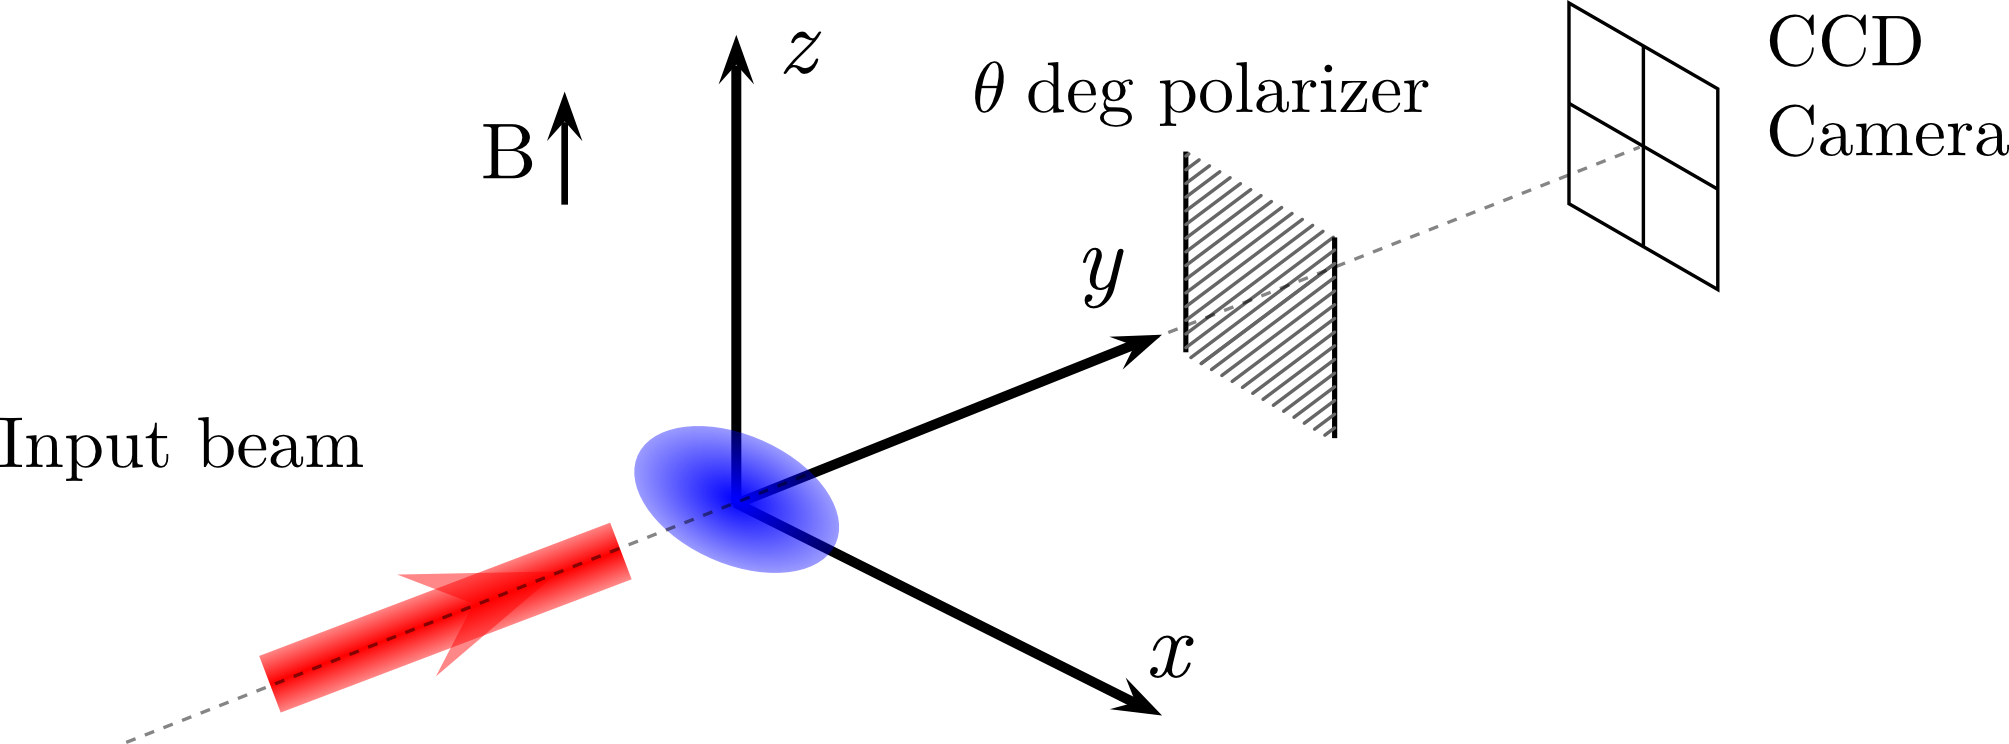
\includegraphics[width=0.85\textwidth]{../figures/phasecon/phase_contrast_02.png}
\caption[Schematic for polarization phase-contrast imaging]{Simple schematic
showing the setup for PPCI.  For simplicity we do not show any of the imaging
optics (lenses and microscope objective) and just include the parts which
affect the polarization of the light.  The atom cloud is represented by the
blue ellipsoid sitting at the origin.  }
\label{fig:phc-setup}
\end{figure}

We use the subscript $f$ to denote the electric field parameters after the
light has interacted with the atom cloud: 
\begin{equation}
 \tilde{\efield}_{f}= 
      \mathcal{E}_{0f} e^{i(\bv{k}\cdot\bv{r} - \omega t + \varphi_{f} )} 
     [ \cos\phcChi_{f} \bv{\hat{e}}_{1} 
   +   \sin\phcChi_{f} e^{i\phi_{f}} \bv{\hat{e}}_{2} ]
\end{equation}


As shown in Fig.~\ref{fig:phc-setup},  after passing through the atom cloud, the
light is passed through a polarizer with transmission axis at an angle
$\theta$, measured with respect to the magnetic field axis. The resulting field
after the polarizer is 
\begin{equation}
  \tilde{\efield}_{\text{pol}} = 
     \mathcal{E}_{0f} e^{i(\bv{k}\cdot\bv{r} - \omega t + \varphi_{f} )} 
     ( \cos\phcChi_{f}\sin\theta  
   +   \sin\phcChi_{f} e^{i\phi_{f}} \cos\theta ) \bv{\hat{e}}_{\theta} 
\label{eq:fieldpol}
\end{equation}
The polarizer thus sums (interferes) the two complex amplitudes corresponding
to $\hat{\bv{e}}_{1,2}$.  The light is then imaged onto a CCD, which is
sensitive only to intensity.  The intensity
at the CCD is given by 
\begin{equation}
\begin{split}
  I_{A}  & = | \tilde{\efield}_{\text{pol} } |^{2}  \\
    & = \mathcal{E}_{0f}^{2}
        ( \cos\phcChi_{f} \sin\theta 
             + \sin\phcChi_{f} \cos\theta \cos\phi_{f} )^{2}
    ~+~ \mathcal{E}_{0f}^{2}(\sin\phcChi_{f} \cos\theta \sin\phi_{f} )^{2} \\ 
    & = \mathcal{E}_{0f}^{2}
        ( \cos( \phcChi_{i}+\delta\phcChi) \sin\theta 
         + \sin( \phcChi_{i} + \delta\phcChi) 
           \cos\theta \cos(\phi_{i} + \delta\phi ))^{2} \\ 
    & ~~~~~~~~~~~~~~~~~~~~~~~~~~~~~~~~~~~~~~~~~~~~~~~~~~
      +~  \mathcal{E}_{0f}^{2}(\sin( \phcChi_{i} +
          \delta\phcChi) \cos\theta \sin( \phi_{i} + \delta\phi) )^{2} \\
    & = \mathcal{E}_{0f}^{2} 
       \left( \cos^{2}(\zeta_{i}+\delta\zeta) \sin^{2}\theta +  
              \sin^{2}(\zeta_{i}+\delta\zeta) \cos^{2}\theta +
         \frac{1}{2} \cos(\phi_{i}+\delta\phi) 
                     \sin(2[\zeta_{i}+\delta\zeta]) \sin(2\theta) \right)
\end{split}
\label{eq:intpol}
\end{equation}
In the last two lines we have expressed the final field parameters in terms of their
initial values and the change, $\delta$, that they undergo after traversing the
cloud.  We note that Eqs.~\ref{eq:fieldpol} and \ref{eq:intpol} are equivalent
to Eqs.  6.2.14 and 6.2.17  in  Curtis Bradley's Ph.D.
thesis~\cite{Bradley1996}. 


If one repeats the analysis, but without atoms, only considering the effect of
the polarizer, one obtains at the CCD:
\begin{equation}
\begin{split}
  I_{N}  & = | \tilde{\efield}_{\text{i} } |^{2}  \\
    & = \efieldo^{2}
        ( \cos\phcChi_{i} \sin\theta + \sin\phcChi_{i} \cos\theta \cos\phi_{i} )^{2}
      +  \efieldo^{2}(\sin\phcChi_{i} \cos\theta \sin\phi_{i} )^{2} \\  
    & = \efieldo^{2} 
       \left( \cos^{2}\zeta_{i} \sin^{2}\theta +  
              \sin^{2}\zeta_{i} \cos^{2}\theta +
         \frac{1}{2} \cos\phi_{i}
                     \sin(2\zeta_{i}) \sin(2\theta) \right)
\end{split}
\end{equation}

In practice one takes a picture with atoms and another picture without atoms, 
and defines the contrast as:
\begin{equation} 
 \frac{ I_{A} - I_{N} }{I_{N}} 
\end{equation} 
We would like to maximize the contrast $(I_{A} - I_{N})/I_{N}$ for a given
change in the field parameters.   

Expanding the expression for $I_{A}-I_{N}$ in the small parameter $\delta\phi$
(and for the moment assuming that $\delta\phcChi = 0$, and
$\mathcal{E}_{0f}=\efieldo$) yields\footnote{Assuming no change in
$\delta\phcChi$ and $\efieldo$ is  justifiable, since both $\delta\phcChi$ and
$\delta( \ln\efieldo)$ are $\propto \xi_{zz} \sim 1/\Delta_{\pi}$, whereas
$\delta\phi$ is proportional to $\xi_{xx} \sim 1/\Delta_{-}$, and therefore we
expect $\delta\phi > \delta(\ln\efieldo), \delta\phcChi$.  }.
\begin{equation} I_{A} - I_{N} \approx -
\frac{\efieldo^{2}}{2} \sin( 2\phcChi) \sin( 2\theta ) \sin(\phi)	\delta \phi
\label{eq:phc-small}
\end{equation} 
Looking at expression~\ref{eq:phc-small} for small $\delta\phi$ points at the
choice for maximizing the contrast: $\phcChi=\theta = \pi/4$ and
$\phi=\pi/2$.   This corresponds to having circularly polarized light at the
input and placing the transmission axis of the polarizer at $45^{\circ}$ from
the magnetic field axis.  

%At this point we digress slightly to elaborate on a technicality that came up
%when we implemented phase contrast imaging:  The values $\phcChi=\theta=\pi/4$
%are easy for a practical implementation of the setup,  the simple analysis
%above tells us that the contrast should be maximized at these values, but it
%turns out 

%  In the lab, one typically uses
%linearly polarized light and a  $\lambda/4$ waveplate  to obtain the
%circularly polarized light.  One can, in principle, maximize the contrast by
%repeatedly imaging equivalent samples and tuning the angles of the $\lambda/4$
%waveplate and the angle, $\theta$, of the polarizer with respect to the
%magnetic field.  If $\theta$ is already known to be $\theta=45^{\circ}$, then
%%This is shown in Fig.~\ref{fig:phc-setup2}.  \begin{figure} \centering
%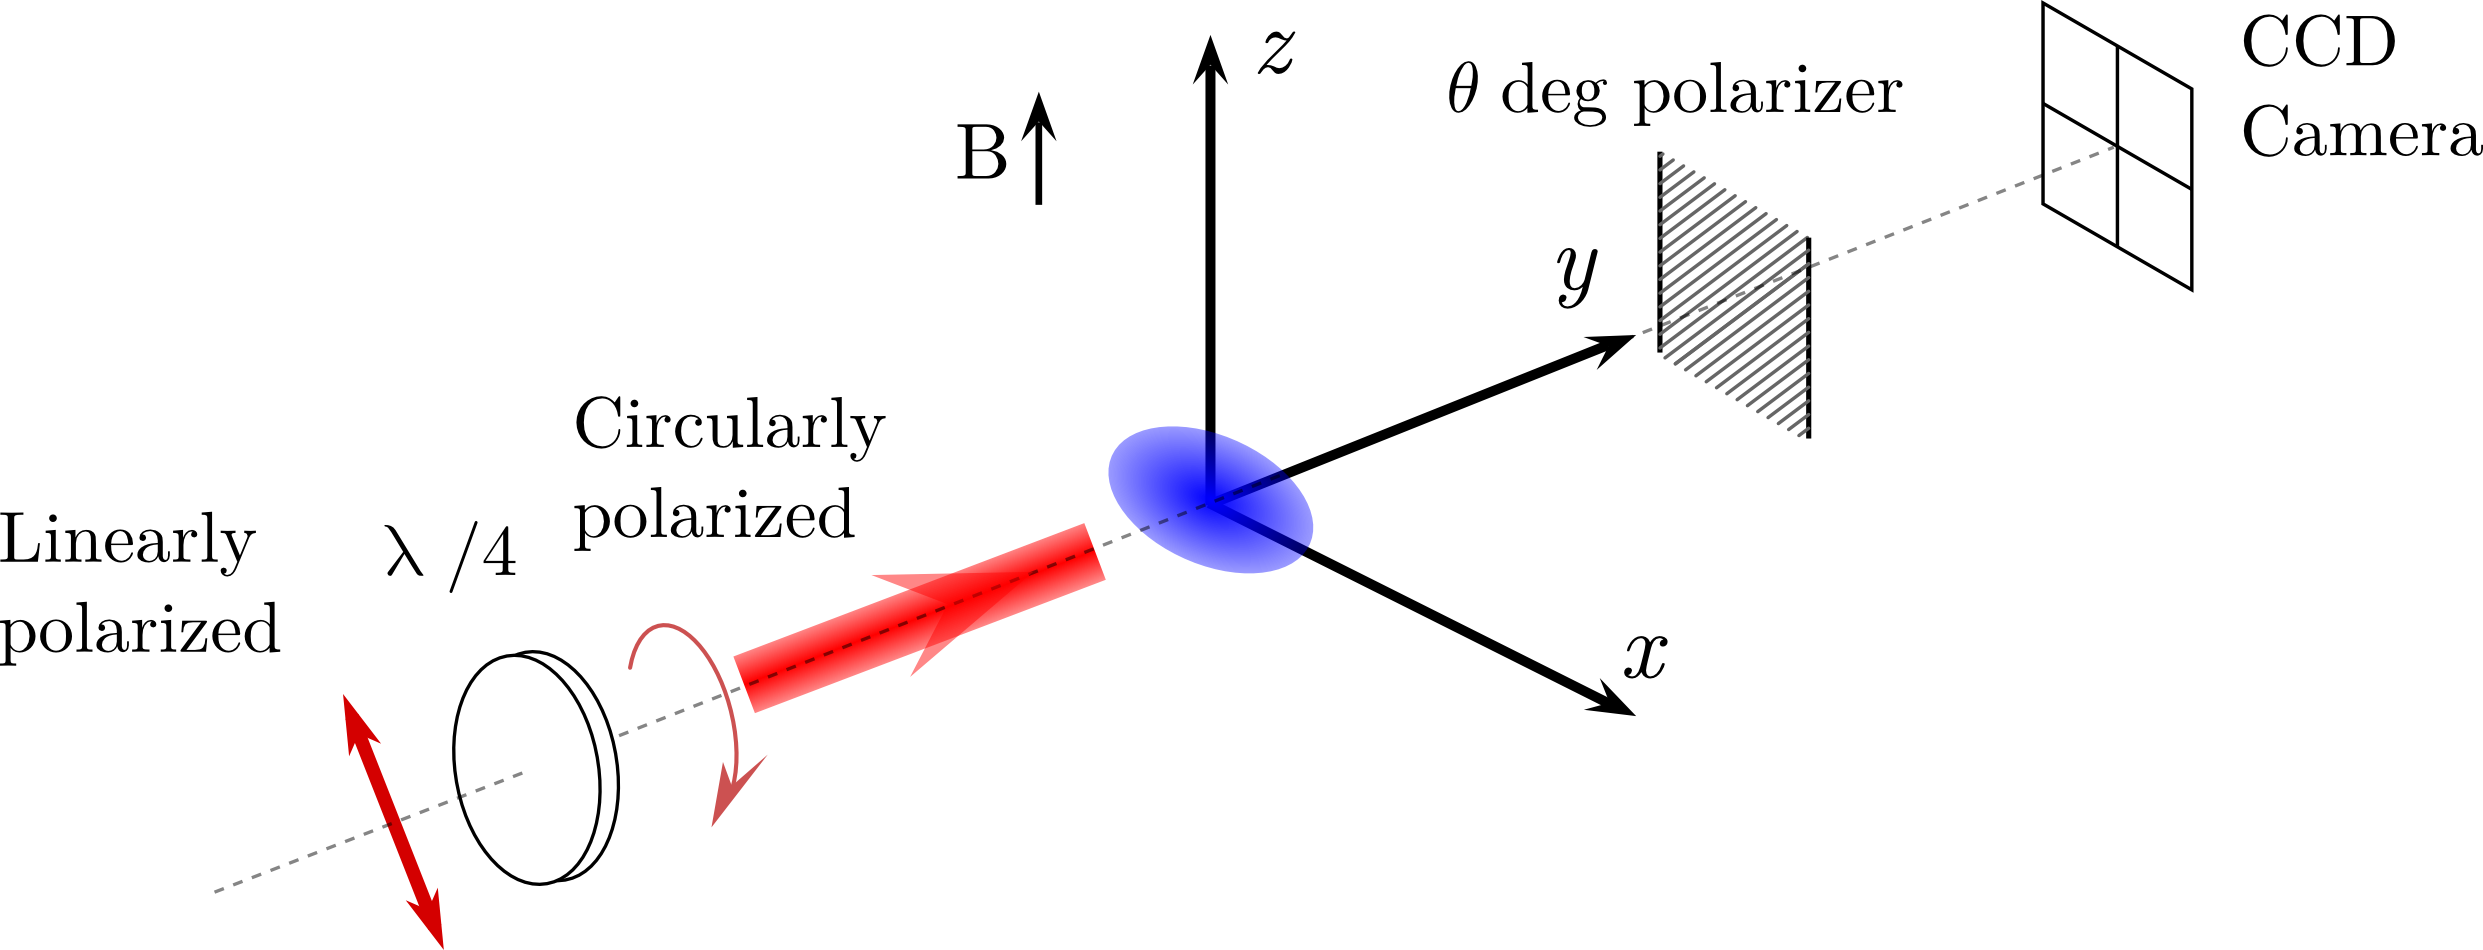
\includegraphics[width=0.85\textwidth]{../figures/phasecon/phase_contrast_03.png}
%\caption[Schematic for polarization phase-contrast imaging]{Simple schematic
%showing the setup for PPCI.   } \label{fig:phc-setup} \end{figure}
 

Having made this choice we go back to the equations for $I_{A}$ and $I_{N}$ and
obtain for the contrast 
\begin{equation}
\begin{split}
  \frac{ I_{A} - I_{N}}{I_{N}}  & =  
     - 1 
     + \left(\frac{ \mathcal{E}_{0f} }{\efieldo}\right)^{2} 
      \left[ 1 -\cos(2\delta\phcChi) \sin(\delta\phi)  \right] \\ 
     \vspace{0.5em}
     & = - 1 
     + e^{2\delta(\ln\efieldo)} 
      \left[ 1 -\cos(2\delta\phcChi) \sin(\delta\phi)  \right]
\end{split}
\end{equation}

Since the parameter changes $\delta(\ln\efieldo)$, $\delta\phcChi$, and 
$\delta\phi$ are all small, we have to first order 
\begin{equation}
  \frac{ I_{A} - I_{N}}{I_{N}}  \approx  
     \delta \phi
\end{equation}

Plugging in the initial values for the field parameters ($\zeta_{i}=\pi/4$ and
$\phi_{i}=\pi/2$) into Eqs.~\ref{eq:delta-field-params} we obtain
\begin{equation}
\begin{split}
 \delta( \ln\efieldo ) & = \ 
      -\frac{1}{2} [ \text{Im}\xi_{xx} + \text{Re}\xi_{zz} ] n_{\text{col}}\\ 
 \delta\varphi & = \
      -\text{Re}\xi_{xx} n_{\text{col}} \\ 
 \delta\phcChi & = \ -\frac{1}{2} 
     [ \text{Im}\xi_{xx}  - \text{Re}\xi_{zz}  ] n_{\text{col}}\\
 \delta\phi & = \
     -[ \text{Re}\xi_{xx} + \text{Im}\xi_{zz} ] n_{\text{col}}, 
\end{split}
\end{equation}
and finally the expression that relates the measured contrast with the column
density: 
\begin{equation}
\begin{split}
  \frac{ I_{A} - I_{N}}{I_{N}}   
     & = - 1 
     + e^{  -[ \text{Im}\xi_{xx} + \text{Re}\xi_{zz} ] n_{\text{col}} } 
      \left[ 1 
        +\cos( [ \text{Im}\xi_{xx} - \text{Re}\xi_{zz} ] n_{\text{col}} ) 
         \sin( [ \text{Re}\xi_{xx} + \text{Im}\xi_{zz} ] n_{\text{col}} )  \right]
\end{split}
\label{eq:final-contrast}
\end{equation}
where $\xi_{xx}$ and $\xi_{zz}$ were defined in Eq.~\ref{eq:def-xis} as  
\begin{equation}
\begin{split}
   \xi_{xx} & = 
    \frac{ 3  \Gamma \lambda^{2}}{ 2 \pi}
       \left( \frac{1/4}{2\Delta_{-} - i \Gamma } 
            + \frac{1/12}{2\Delta_{+} - i \Gamma }  
       \right)  \\
   \xi_{zz} & = 
    \frac{ 3  \Gamma \lambda^{2}}{ 2 \pi}
              \frac{1/3}{2\Delta_{\pi} - i \Gamma } 
\end{split}
\end{equation}

Equation~\ref{eq:final-contrast} can be inverted numerically to recover the
column density from a measured value of the contrast.

\subsection{ Results } 

To conclude the chapter on phase-contrast imaging, we show how the
consideration of other excited states affects a measurement of  the total atom
number.  We prepare a sample in our optical dipole trap, and image it
\textit{in-situ} using different values of the imaging detuning.
Figure~\ref{fig:phc-number} shows that we get the same atom number (as
expected) only if the analysis includes the contribution from all the excited
states.  We also verified that the absolute scale of the atom number was
correct by independently determining the atom number using strong saturation
absorption imaging~\cite{reinaudi2007strong}.   For detunings close to
resonance with state $|2\rangle$, the phase-contrast analysis breaks down
because the detuning and the linewidth become comparable and the interaction of
the light can not longer be described as purely dispersive.
\begin{figure}
\centering
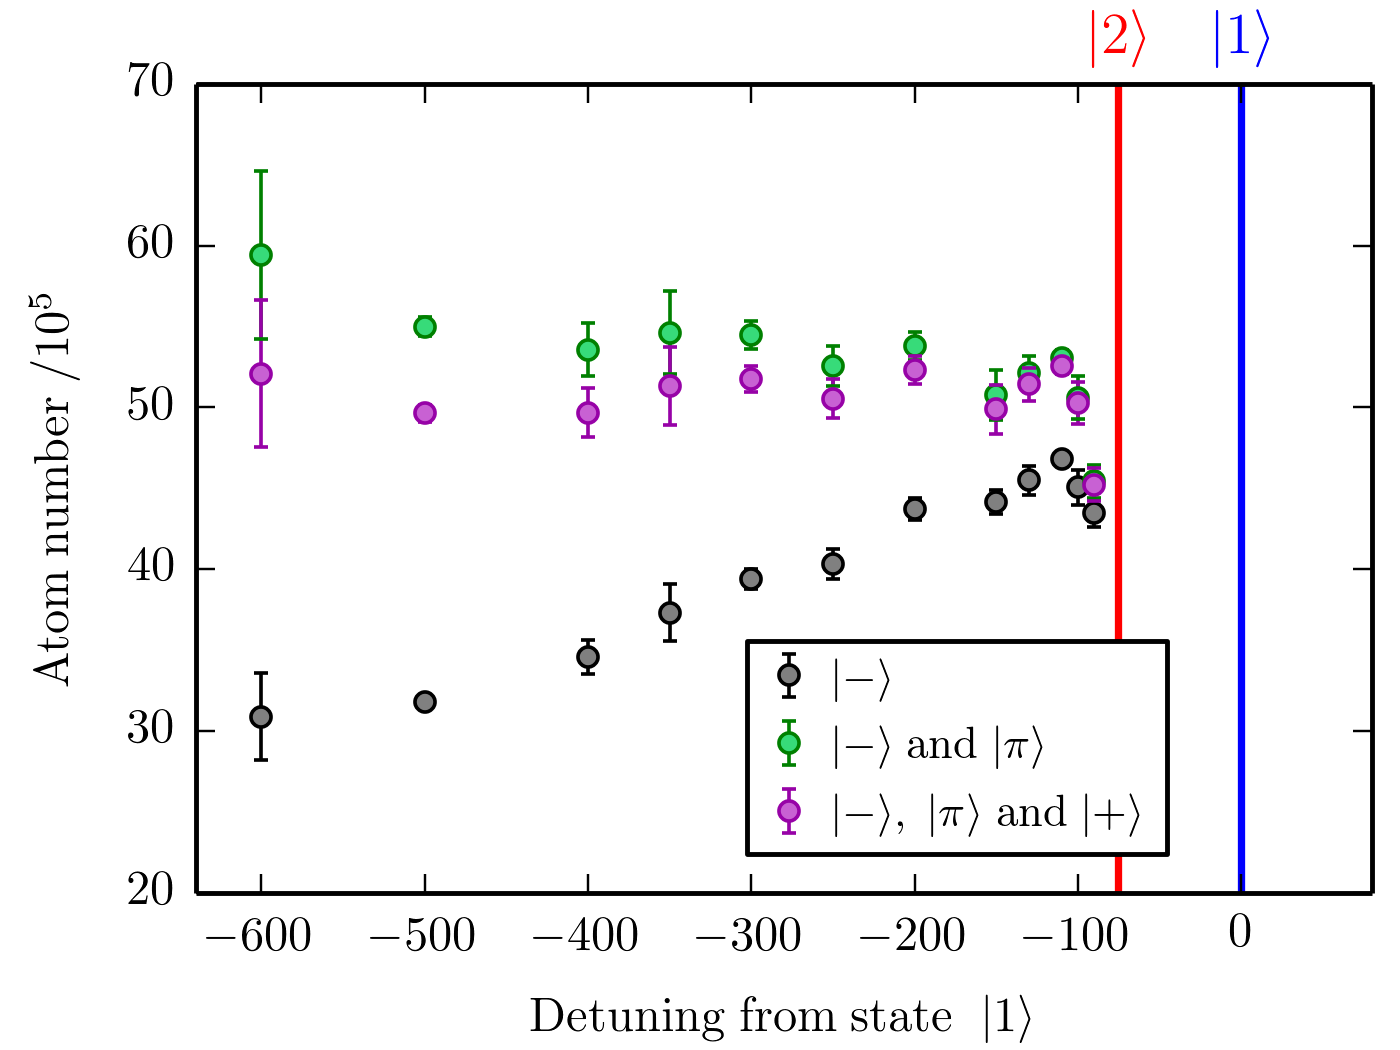
\includegraphics[width=0.8\textwidth]{../figures/phasecon/phc-numberVSdet_thesis.png}
\caption[Phase-contrast imaging vs. detuning]{Total atom number obtained from
polarization phase-contrast imaging.  The different points show analyses of the
contrast signal using contributions from one (black), two (green), and three
(purple) of the excited states.  Only if we include all three contributions we
obtain, as expected, a measurement which is independent of the imaging light
detuning. }
\label{fig:phc-number}
\end{figure}


%%%%%%%%%%%%%%%%%%%%%%%%%%%%%%%%%%%%%%%%%%%%%%%%%%%%%%%%%%%%%%%%%%%%%%%%%%%%%%%
%%%%%%%%%%%%%%%%%%%%%%%%%%%%%%%%%%%%%%%%%%%%%%%%%%%%%%%%%%%%%%%%%%%%%%%%%%%%%%%
%%%%  CHAPTER 7
%%%%%%%%%%%%%%%%%%%%%%%%%%%%%%%%%%%%%%%%%%%%%%%%%%%%%%%%%%%%%%%%%%%%%%%%%%%%%%%
%%%%%%%%%%%%%%%%%%%%%%%%%%%%%%%%%%%%%%%%%%%%%%%%%%%%%%%%%%%%%%%%%%%%%%%%%%%%%%%
\chapter{Diagnostic tools II: Fermi gas thermometry}
\label{chap:fermi-thermometry}


The starting point for all of our experiments is a deeply degenerate Fermi gas
at a temperature $T\approx 0.04 T_{F}$, where $T_{F}$ is the Fermi temperature.
This degenerate sample is created in a harmonic trapping potential, and from
there we slowly ramp up the optical lattice potential, where final measurements
take place.  Measuring the $T/T_{F}$ ratio in a harmonic trap is an important
part of our experiment.  Most of the time in the lab is spent optimizing the
performance of the apparatus, so that the lowest temperatures can be reached in
the dimple trap and we can proceed with experiments in the optical lattice.  To
obtain $T/T_{F}$, we image the column density distribution of the atomic gas
and fit its shape to a Thomas-Fermi distribution.   This procedure is well
documented in the literature~\cite{Making2007}, and pretty much every PhD
thesis on ultracold Fermi gases has something to say about it. This one is no
exception.   

The main contribution from this work to the process of Fermi thermometry in our
lab has been in the creation of high-performance fitting routines to enable
feedback to the experimenter on a time scale faster than the repetition rate of
the experimental cycle.  The performance bottleneck in the fitting algorithm is
the evaluation of the Fermi-Dirac integral (or polylogarithm),  a special
function that describes the shape of the density distribution at low
temperatures (as we will see below).  The imaging process produces a
two-dimensional (2D) column density distribution, however, previous experiments
in the lab fitted cuts over the distribution, or sums over it in order to
have the fitting routine handle the easier one-dimensional (1D) fitting
problem.  

In our work, we started by exploring 2D surface fits of the column density in
order to gain advantage of all of the information contained in the measurement.
We first implemented fitting routines in Python but found that it would take up
to several minutes to fit a single image.    We then developed fitting routines
using C++ , the GNU Scientific
Library\footnote{http://www.gnu.org/software/gsl/}, and a simple for-loop
parallelization using OpenMP.  This cut down the fitting time to single digit
seconds.   The duty cycle in our experiment is $\sim20-30$ s, so
the new fitting routines allowed us to gain immediate feedback on the
temperature of the sample.

The substance of our contribution is of course in the code itself, which is
archived on the web and available for download at~\cite{PedroMDuarte:11760}.  In this
section we outline the derivation of the fitting functions that are implemented
in the code.  


\subsection{Density distributions of a trapped Fermi gas}

In the Thomas-Fermi approximation one considers the number density of the gas
in phase space, $w(\vec{r},\vec{p})$:
\begin{equation}
w(\vec{r},\vec{p}) = 
    \frac{1}{(2\pi\hbar)^{3}} 
    \frac{1}{\exp\left[\beta(\vec{p}^{2}/2m + V(\vec{r}) - \mu) \right] + 1 }  
%    \equiv \frac{1}{(2\pi\hbar)^{3}} f(\vec{r},\vec{p})
\end{equation}
The density distribution of the trapped gas can be obtained by integrating the
phase space density over momentum space~\cite{Butts1997}.  For example, at
zero temperature, where the energy dependence of the number density is the
usual Fermi step function,  the profile takes the shape of the trapping
potential elevated to the 3/2 power:
\begin{equation}
  n(\vec{r}) = \int w(\vec{r},\vec{p})\mathrm{d} \vec{p}~
    \overset{T\to 0 }{\longrightarrow}  
    \int_{| \vec{p}| < \sqrt{2m(\mu-V(\vec{r}))}} i
          \frac{\mathrm{d} \vec{p}}{(2\pi\hbar)^{3}} 
 = \frac{1}{6\pi^{2}} \left( \frac{2m}{\hbar^{2}} \right)^{3/2}
               (\mu - V(\vec{r}))^{3/2}
\end{equation}
In a harmonic trap at zero temperature the density distribution is
\begin{equation}
n(\vec{r}) = \frac{8}{\pi^{2}} 
             \frac{N}{\rf{x} \rf{y} \rf{z}} 
\left[ \max\left( 1 - \sum_{i} \frac{x_{i}^{2}}{\rf{i}^{2}} , 0 \right) \right]^{3/2} ,
\end{equation}
where the Fermi radius is defined as $\rf{i} = \sqrt{\frac{ 2 E_{\mathrm{F}}}{m
\omega_{i}^{2}}}$. 

At a finite temperature, one can carry out the integral by first changing to
dimensionless momentum $\vec{q} = \sqrt{\frac{\beta}{2m}}\vec{p}$ and then
changing variables to replace the magnitude of $\vec{q}$ as $w=q^{2}$:
\begin{equation}
\begin{split}
  n(\vec{r}) =  \int w(\vec{r},\vec{p}) \,\mathrm{d}\vec{p}  = &
  \frac{\left( 2m/\beta \right)^{3/2}}{(2\pi\hbar)^{3}} 
    \int \frac{\mathrm{d}\vec{q}}{\exp\left[ q^{2} - (\mu -V(\vec{r}))\beta \right] + 1 } \\
   =  &
  \frac{1}{\ldb^{3}}  \frac{ 1 } { \Gamma(3/2)} 
  \int_{0}^{\infty} 
   \frac{w^{1/2}}{\exp\left[ w - (\mu - V(\vec{r}))\beta \right] +1 } 
   \,\mathrm{d} w.
\end{split}
\label{eq:dens-integral}
\end{equation}
Here we have introduced the thermal de Broglie wavelength, $\ldb =
\frac{h}{\sqrt{2\pi m \kb T}}$, and used the Gamma function (rather than the
usual $4\pi$) to represent the surface area of the sphere\footnote{The surface
area of an $n$-shell with radius $R$ and thickness $\mathrm{d}R$ is given by
$\frac{2 \pi^{n/2}}{\Gamma(n/2)} R^{n-1} \mathrm{d} R$} This allows us to
readily identify the integral on the right as a Fermi-Dirac integral or a
polylogarithm.  These two special functions are defined as follows:  
\begin{align} 
  n^{\mathrm{th}}-\mathrm{order\ Polylogarithm} & &  
   \pli_{n} (z) &= \frac{1}{\Gamma(n)} 
   \int_{0}^{\infty} \mathrm{d} q \frac{ q ^{n-1} }{ e^{q}/z -1 } \\
  j^{\mathrm{th}}-\mathrm{order\ Fermi-Dirac\ Integral} &  &   
    F_{j}(z) &=  \frac{1}{\Gamma(j+1)} 
   \int_{0}^{\infty} \mathrm{d} t  \frac{ t^{j} } { e^{t-z} + 1}  \\
\end{align}
Different authors pick the polylogarithm or the Fermi-Dirac function,  they are
equivalent to each other in the following way:
\begin{equation}
  F_{n}(z) = -\pli_{n+1}(-e^{z}) 
\end{equation}
Here we use the Fermi-Dirac integral notation, for the simple reason that this
function is readily available in the GNU Scientific Library.  The reader can
use the equivalence relation to go back to the polylog notation when necessary.
The density of the thermal gas in Eq.~\ref{eq:dens-integral} can then be simply
written as
\begin{equation}
n(\vec{r}) = \ldb^{-3} F_{1/2}( \beta[\mu - V(\vec{r})])
\label{eq:dens-fermi} 
\end{equation}

\subsection{Time-of-flight}

If the cloud is suddenly released from the trapping potential, the density
distribution at time $t$ after the release can be written as
\begin{equation}
  n(\vec{r},t) = 
%   \int \mathrm{d} \vec{r}_{0} 
%    \int \frac{ \mathrm{d} \vec{p}_{0}} { (2\pi\hbar)^{3}} 
%       f(\vec{r}_{0} , \vec{p}_{0}) \delta( \vec{r} - \vec{r}_{0} - \vec{p}_{0}\, t/m)  
     \int w(\vec{r} - \vec{p}_{0}t/m,\vec{p}_{0} )\,\mathrm{d} \vec{p}_{0}
%\frac{ \mathrm{d} \vec{p}_{0}} { (2\pi\hbar)^{3}} 
%       f(\vec{r} - \vec{p}_{0}\,t/m , \vec{p}_{0}) 
\end{equation}
Here we neglected the interactions between the particles.  Experimentally, we
use a magnetic Feshbach resonance which allows us to control the scattering
length between \li\ atoms in two different hyperfine
states~\cite{Houbiers1998}.  The Feshbach resonance allows us to set the
scattering length to zero, such that the collision cross section vanishes and
the the cloud expands ballistically. 

The integration over momentum, which we performed easily in
Eq.~\ref{eq:dens-integral} could be complicated because the momentum now
appears inside the potential energy as  $V(\vec{r}-\vec{p}_{0} t/m)$.   A
harmonic trapping potential has a quadratic dependence on position, and one
finds that the integral is easy to carry out with a change of variables.  If
the potential has trapping frequencies $\omega_{i}$ such that  
\begin{equation} 
 V(\vec{r}) =  \sum_{i} \frac{1}{2} m \omega_{i}^{2} r_{i}^{2} 
\end{equation}
then one finds for the density after time-of-flight (TOF) 
\begin{equation}
  n(\vec{r},t) = 
  \ldb^{-3} \left(\prod_{i} (1 + \omega_{i}^{2}t^{2})^{-1/2} \right) 
   F_{1/2}\left( \beta\left[ \mu -
   \sum_{i}\frac{1}{2} m \frac{\omega_{i}^{2}}{1+ \omega_{i}^{2} t^{2}} 
     x_{i}^{2} \right] \right)
\label{eq:001}
\end{equation}
For the harmonic potential this is the same functional form as in
Eq.~\ref{eq:dens-fermi}, except the lengths are rescaled as 
\begin{equation}
  x_{i}^{2}  \rightarrow  \frac{ x_{i}^{2}}  {1+ \omega_{i}^{2} t^{2}}
\end{equation} 
In this case the expansion is said to be self-similar, because the shape of the
density distribution never changes as the cloud expands.   Since we determine
the ratio $T/T_{F}$ from fitting the shape of the cloud,  for a harmonic
potential this can be done \textit{in-situ} or after TOF.  

Practically there are two advantages from performing thermometry after TOF.  As
we saw in the previous section, having a very large optical density requires
large detunings to stay within the dispersive requirements for phase-contrast
imaging.  As the atoms expand their density is reduced and eases those
requirements.  The second reason, is that the features of the shape of the
distribution, which will reveal the temperature of the gas,  now occupy a
larger number of pixels in the image.  In other words, the expansion provides
more resolution at no cost.  


\subsection{Column density and imaging geometry}

In our experiment we take phase-contrast images in one of three traps:  the
crossed-beam optical dipole trap (ODT), the dimple trap or the optical lattice.
The dimple and optical lattice are nearly spherically symmetric, but the ODT is
highly elongated.   Using the principal axes of the ODT we define a coordinate
system, as shown in Fig.~\ref{fig:geometry}.  The direction of propagation of
the imaging light is not along any of the principal axes, so we define the
directions $c$ and $g$ which go along the imaging direction and perpendicular
to it, respectively.  
\begin{figure}
\centering 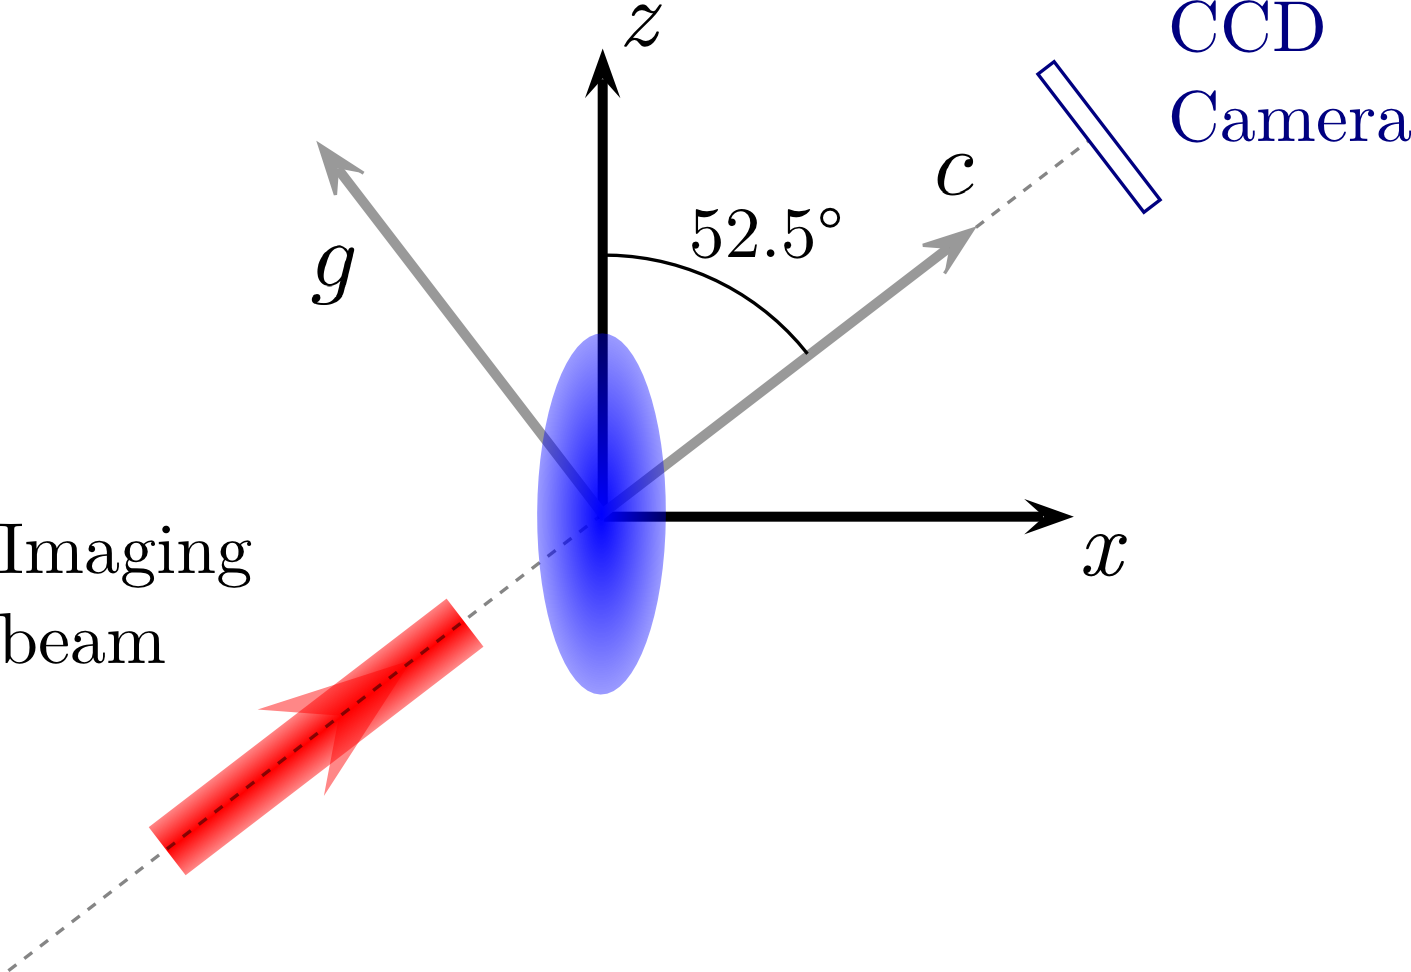
\includegraphics[width=0.5\textwidth]{../figures/fermi-thermometry/camera_setup.png}
\caption[Camera axis geometry]{Camera axis is at 52.5$^{\circ}$ from $z$.  New axes $c$ and $g$ are defined, $y$ remains the same.   The shorthand notation $\alpha = \cos(52.5^{\circ})$ and $\gamma = \sin(52.5^{\circ})$ is used.}  \label{fig:geometry}
\end{figure}

The column density that we record when imaging the cloud corresponds to the
integral along $c$:
\begin{equation}
\int  n( \vec{r}, t) \,\mathrm{d} c
\end{equation} 
Since we wish to keep the information regarding the trap frequencies, which are
measured along the principal axes of the ODT we derive here formulas for the
column density of the cloud when imaging along the $c$ direction.  We define
the following notation:
\begin{align}
 \alpha & = \cos(52.5^{\circ}) & \gamma & = \sin(52.5^{\circ}) \\ 
J_{i} & = \frac{\omega_{i}^{2}}{1+\omega_{i}^{2} t^{2}} & 
M & = \sqrt{ \gamma^{2} J_{x} + \alpha^{2} J_{z} } \\
N & =  \frac{\alpha \gamma (J_{z} - J_{x}) }{M} & 
J_{g} & = \alpha^{2} J_{x} + \gamma^{2} J_{z} - N^{2}
\end{align}
We can write down the phase-space density as 
\begin{equation}
w(p,c,g,y) = \frac{1}
      {\exp\left[ \frac{\beta p^{2}}{2m} - \beta\mu + 
   \frac{m\beta}{2}( (M c + Ng)^{2}+ J_{g}g^{2} + J_{y} y^{2} ) \right] + 1   }
\end{equation}
and the column density becomes 
\begin{equation}
n_{\mathrm{col}}(g,y,t) = 
    \frac{ 1 } { (2\pi\hbar)^{3}}  
  \left(\prod_{i} (1 + \omega_{i}^{2}t^{2})^{-1/2} \right) 
   \int w(p,c,g,y)\,\, \mathrm{d} \vec{p}\, \mathrm{d}{c} 
\label{eq:ncol_int}
\end{equation}
The following change of variables: $s=\sqrt{\beta/2} (M c + Ng)$  and $\vec{p'}
= \sqrt{\beta/(2m)} \vec{p}$\,,  allows us to carry out the integral, by
exploiting the four-dimensional symmetry in $(\vec{p'},s)$-space and using 
\begin{equation}
\int \mathrm{d} \vec{p}\, \mathrm{d}{c} = 
   \left(\frac{2}{\beta}\right)^{2}\frac{m}{M} 
       \int \mathrm{d} \vec{p'}\, \mathrm{d}{s} 
   = \left(\frac{2}{\beta}\right)^{2}\frac{m}{M} 
    \int  \frac{2 \pi^{2}}{\Gamma(2)} R^{3} \mathrm{d} R
\end{equation}
where $R$ is the radius of the 4D sphere defined by $p'^{2} + s^{2} = R^{2}$.
We obtain
\begin{multline}
n_{\mathrm{col}}(g,y,t) =  
  \frac{ 1 } { (2\pi\hbar)^{3}}  
   \left(\prod_{i} (1 + \omega_{i}^{2}t^{2})^{-1/2} \right)  
  \left(\frac{2}{\beta}\right)^{2}\frac{m}{M}  
  \times  \\  \int  \frac{R^{3}}{\exp\left[ R^{2} - \beta\mu 
      + \frac{m\beta}{2}( J_{g}g^{2} + J_{y} y^{2} ) \right] + 1   } 
      \frac{ 2\pi^{2} \mathrm{d} R}{\Gamma(2)}
\end{multline}
A final change of variables to $q = \sqrt{R}$ gives
\begin{multline}
n_{\mathrm{col}}(g,y,t) =  
   \frac{ 1 } { (2\pi\hbar)^{3}}  
   \left(\prod_{i} (1 + \omega_{i}^{2}t^{2})^{-1/2} \right)  
  \left(\frac{2}{\beta}\right)^{2}\frac{\pi^{2} m}{M} \times \\ 
   \int  \frac{q}{\exp\left[ q - \beta\mu 
     + \frac{m\beta}{2}( J_{g}g^{2} + J_{y} y^{2} ) \right] + 1   } 
   \frac{\mathrm{d} q }{\Gamma(2)}
\end{multline}
where the Fermi-Dirac integral can be spotted again (this time of order 1
rather than 1/2) to yield
\begin{equation}
n_{\mathrm{col}}(g,y,t) =  \frac{ 1 } { (2\pi\hbar)^{3}}  
   \left(\prod_{i} (1 + \omega_{i}^{2}t^{2})^{-1/2} \right)  
   \left(\frac{2}{\beta}\right)^{2}\frac{\pi^{2} m}{M} F_{1} 
   \left( \beta\mu  - \frac{m\beta}{2}  ( J_{g}g^{2} + J_{y} y^{2} )\right)
\label{eq:ncol-fun} 
\end{equation}
At zero temperature this becomes: 
\begin{equation}
n_{\mathrm{col,T=0}}(g,y,t) =  
  \frac{ 1 } { (2\pi\hbar)^{3}} 
   \left(\prod_{i} (1 + \omega_{i}^{2}t^{2})^{-1/2} \right) 
    \frac{m}{M}  \frac{ 2\pi^{2}}{\Gamma(2)} 
 \left[ \max\left( \mu - \frac{m}{2}( J_{g}g^{2} + J_{y} y^{2} ) \,\, , \,\,  0 \right) \right]^{2}
\end{equation}


\subsection{Fitting functions}

For the actual fitting routine, we absorb all of the prefactors in front of the
Fermi-Dirac function in Eq.~\ref{eq:ncol-fun} into a fit parameter,
$n_{\mathrm{col},0}$, and also define the cloud radii as 
\begin{align}
 R_{g}^{2} = \frac{F_{0}(\beta\mu)}{F_{-1}(\beta\mu)} 
    \frac{2} {m\beta J_{g}} \\
 R_{y}^{2} = \frac{F_{0}(\beta\mu)}{F_{-1}(\beta\mu)} 
    \frac{2} {m\beta J_{y}} \\
\end{align}
to obtain 
\begin{equation}
n_{\mathrm{col}}(g,y,t) =   
   \frac{n_{\mathrm{col},0}}{ F_{1}(\beta\mu)}   
   F_{1} \left( \beta\mu  -  \frac{F_{0}(\beta\mu)}{F_{-1}(\beta\mu)} 
     \left( \frac{g^{2}}{R_{g}^{2}} + \frac{y^{2}}{R_{y}^{2}} \right)
\right)
\label{eq:ncol}
\end{equation}
The fit parameters are then: $n_{\mathrm{col},0}$, $\beta\mu$, $R_{g}$ and
$R_{y}$.  One can obtain the reduced temperature of the cloud as 
\begin{equation}
T/\TF = (6 F_{2}(\beta\mu) )^{-1/3} 
\label{eq:ncolTTF}
\end{equation} 
Also, if the trap frequencies are known one can obtain the absolute temperature
of the cloud from the sizes long the $g$ and $y$ directions as:
\begin{align}
\kb T_{g} &= 
   m\frac{ \alpha^{2} J_{x} + 
    \gamma^{2} J_{z}- N^{2}}{2} \frac{R_{g}^{2}}{F_{0}(\beta\mu)/F_{-1}(\beta\mu)}
\label{eq:ncolT1} 
 \\
\kb T_{y} &= 
   m\frac{J_{y}}{2} \frac{R_{y}^{2}}{F_{0}(\beta\mu)/F_{-1}(\beta\mu)}
\label{eq:ncolT2} 
\end{align}

In Fig.~\ref{fig:betamu} we show the dependence of $T/T_{F}$ and
$\frac{F_{0}(\beta\mu)}{F_{-1}(\beta\mu)}$ on $\beta\mu$.  
\begin{figure}
\centering
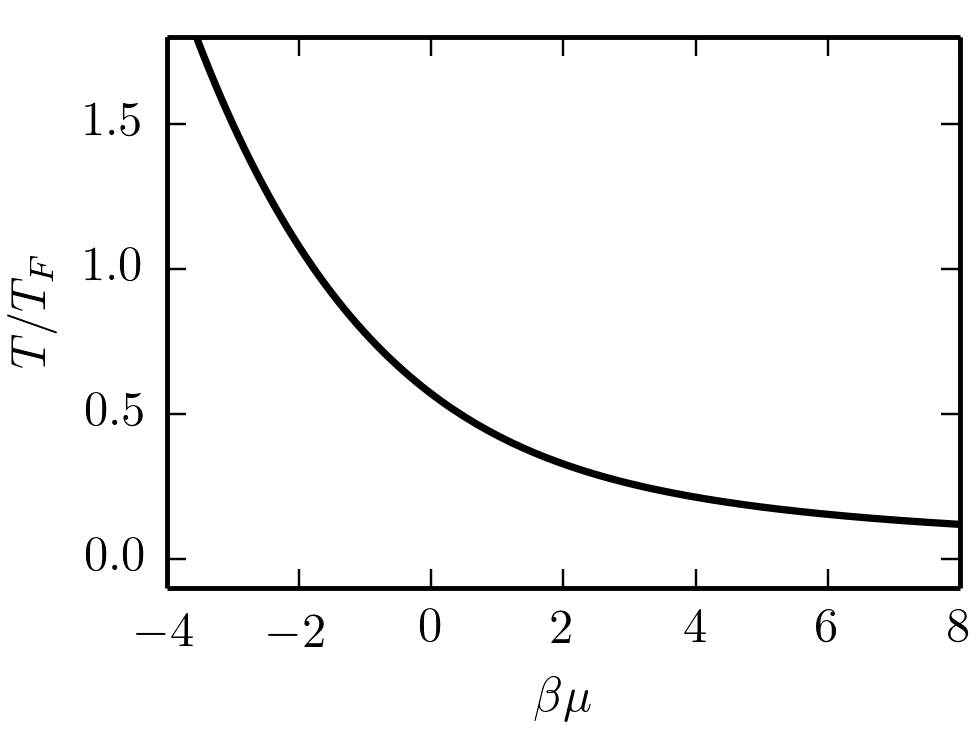
\includegraphics[width=0.45\textwidth]{../figures/fermi-thermometry/tf.png}
~\centering
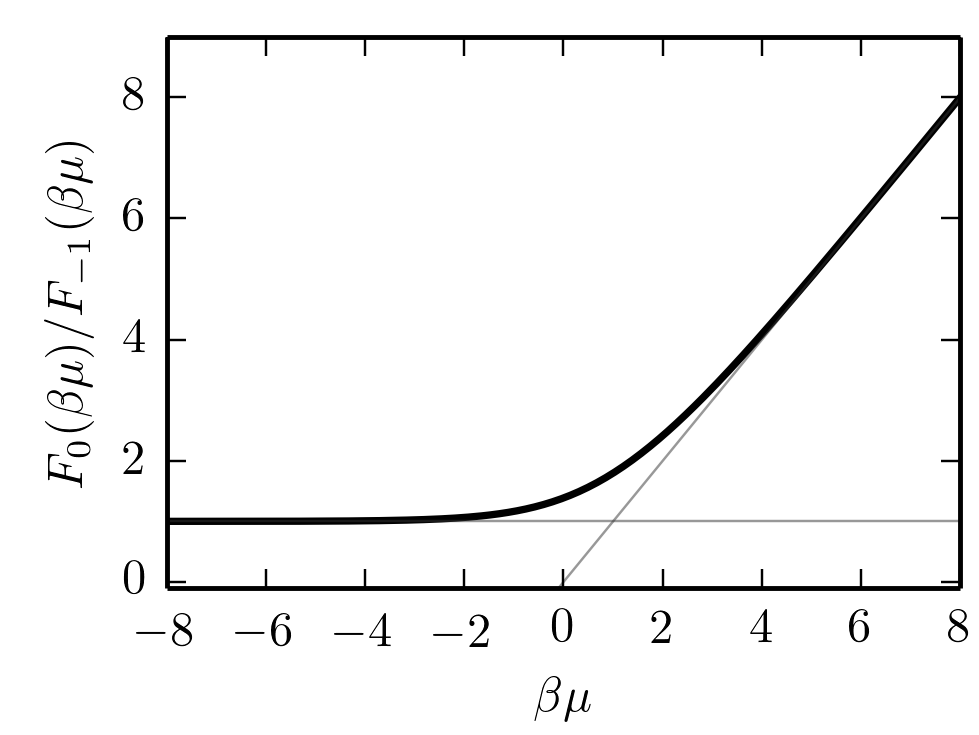
\includegraphics[width=0.45\textwidth]{../figures/fermi-thermometry/fq.png}
\caption[Dependence on $\beta\mu$]{Dependence of $T/T_{F}$ and
$\frac{F_{0}(\beta\mu)}{F_{-1}(\beta\mu)}$ on $\beta\mu$.   For a thermal gas
$\beta\mu<0$ and for a highly degenerate gas $\beta\mu \gg 1 $. }
\label{fig:betamu}
\end{figure}
We see that when the gas is not degenerate ($\beta\mu < 0$) the radius
prefactor,$\frac{F_{0}(\beta\mu)}{F_{-1}(\beta\mu)}$, goes to 1.  This reflect
the fact that in that case the size of the cloud squared is proportional to the
temperature.   On the other hand, for a degenerate gas ($\beta\mu > 0$) the
radius prefactor goes to $\beta\mu$ , which reflects the fact that the size of
the cloud squared is proportional to the Fermi temperature.  More details on
this choice for the fitting function can be found in~\cite{Making2007}.  



